\documentclass{standalone}
\usepackage{tikz}
\usetikzlibrary{patterns, positioning}


\begin{document}
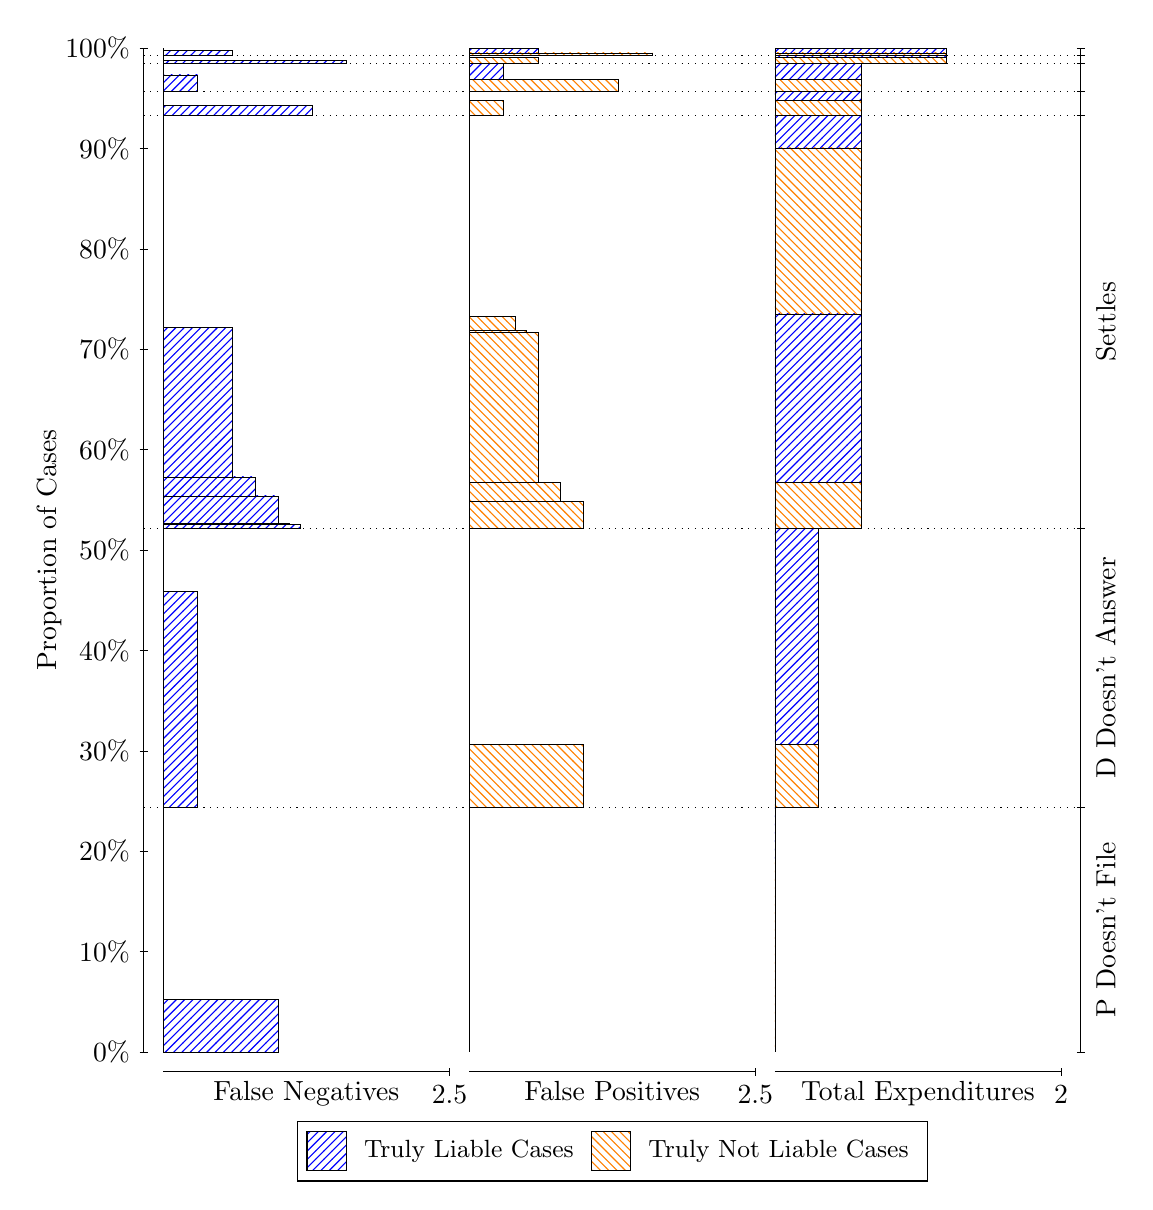
\begin{tikzpicture}
\draw[black, very thin] (1.5,1.75) -- (1.5,14.5);
\node[rotate=90, text=black, anchor=center] at (0.3, 8.125) {Proportion of Cases};
\draw[black, very thin] (1.45,1.75) -- (1.55,1.75);
\node[text=black, anchor=east] at (1.45, 1.75) {0\%};
\draw[black, very thin] (1.45,3.025) -- (1.55,3.025);
\node[text=black, anchor=east] at (1.45, 3.025) {10\%};
\draw[black, very thin] (1.45,4.3) -- (1.55,4.3);
\node[text=black, anchor=east] at (1.45, 4.3) {20\%};
\draw[black, very thin] (1.45,5.575) -- (1.55,5.575);
\node[text=black, anchor=east] at (1.45, 5.575) {30\%};
\draw[black, very thin] (1.45,6.85) -- (1.55,6.85);
\node[text=black, anchor=east] at (1.45, 6.85) {40\%};
\draw[black, very thin] (1.45,8.125) -- (1.55,8.125);
\node[text=black, anchor=east] at (1.45, 8.125) {50\%};
\draw[black, very thin] (1.45,9.4) -- (1.55,9.4);
\node[text=black, anchor=east] at (1.45, 9.4) {60\%};
\draw[black, very thin] (1.45,10.675) -- (1.55,10.675);
\node[text=black, anchor=east] at (1.45, 10.675) {70\%};
\draw[black, very thin] (1.45,11.95) -- (1.55,11.95);
\node[text=black, anchor=east] at (1.45, 11.95) {80\%};
\draw[black, very thin] (1.45,13.225) -- (1.55,13.225);
\node[text=black, anchor=east] at (1.45, 13.225) {90\%};
\draw[black, very thin] (1.45,14.5) -- (1.55,14.5);
\node[text=black, anchor=east] at (1.45, 14.5) {100\%};

\draw[black, very thin] (13.4,1.75) -- (13.4,14.5);
\draw[black, very thin] (13.35,1.75) -- (13.45,1.75);
\node[anchor=west] at (13.35, 1.75) {};
\draw[black, very thin] (13.35,4.8558) -- (13.45,4.8558);
\node[anchor=west] at (13.35, 4.8558) {};
\draw[black, very thin] (13.35,8.3981) -- (13.45,8.3981);
\node[anchor=west] at (13.35, 8.3981) {};
\draw[black, very thin] (13.35,13.647) -- (13.45,13.647);
\node[anchor=west] at (13.35, 13.647) {};
\draw[black, very thin] (13.35,13.952) -- (13.45,13.952);
\node[anchor=west] at (13.35, 13.952) {};
\draw[black, very thin] (13.35,14.309) -- (13.45,14.309);
\node[anchor=west] at (13.35, 14.309) {};
\draw[black, very thin] (13.35,14.408) -- (13.45,14.408);
\node[anchor=west] at (13.35, 14.408) {};
\draw[black, very thin] (13.35,14.5) -- (13.45,14.5);
\node[anchor=west] at (13.35, 14.5) {};

\draw[black, very thin, pattern color=blue, pattern=north east lines] (1.75,1.75) rectangle (3.2033,2.4181);
\draw[black, very thin, pattern color=orange, pattern=north west lines] (1.75,2.4181) rectangle (1.75,4.8558);
\draw[black, very thin, pattern color=blue, pattern=north east lines] (1.75,4.8558) rectangle (2.186,7.5947);
\draw[black, very thin, pattern color=orange, pattern=north west lines] (1.75,7.5947) rectangle (1.75,8.3981);
\draw[black, very thin, pattern color=blue, pattern=north east lines] (1.75,8.3981) rectangle (3.494,8.4516);
\draw[black, very thin, pattern color=blue, pattern=north east lines] (1.75,8.4516) rectangle (3.3487,8.4625);
\draw[black, very thin, pattern color=blue, pattern=north east lines] (1.75,8.4625) rectangle (3.2033,8.812);
\draw[black, very thin, pattern color=blue, pattern=north east lines] (1.75,8.812) rectangle (2.9127,9.0522);
\draw[black, very thin, pattern color=blue, pattern=north east lines] (1.75,9.0522) rectangle (2.622,10.948);
\draw[black, very thin, pattern color=orange, pattern=north west lines] (1.75,10.948) rectangle (1.75,13.647);
\draw[black, very thin, pattern color=blue, pattern=north east lines] (1.75,13.647) rectangle (3.6393,13.767);
\draw[black, very thin, pattern color=orange, pattern=north west lines] (1.75,13.767) rectangle (1.75,13.952);
\draw[black, very thin, pattern color=blue, pattern=north east lines] (1.75,13.952) rectangle (2.186,14.158);
\draw[black, very thin, pattern color=orange, pattern=north west lines] (1.75,14.158) rectangle (1.75,14.309);
\draw[black, very thin, pattern color=blue, pattern=north east lines] (1.75,14.309) rectangle (4.0753,14.339);
\draw[black, very thin, pattern color=orange, pattern=north west lines] (1.75,14.339) rectangle (1.75,14.408);
\draw[black, very thin, pattern color=blue, pattern=north east lines] (1.75,14.408) rectangle (2.622,14.47);
\draw[black, very thin, pattern color=orange, pattern=north west lines] (1.75,14.47) rectangle (1.75,14.5);
\draw[black, very thin, pattern color=orange, pattern=north west lines] (5.6333,1.75) rectangle (5.6333,4.1877);
\draw[black, very thin, pattern color=blue, pattern=north east lines] (5.6333,4.1877) rectangle (5.6333,4.8558);
\draw[black, very thin, pattern color=orange, pattern=north west lines] (5.6333,4.8558) rectangle (7.0867,5.6592);
\draw[black, very thin, pattern color=blue, pattern=north east lines] (5.6333,5.6592) rectangle (5.6333,8.3981);
\draw[black, very thin, pattern color=orange, pattern=north west lines] (5.6333,8.3981) rectangle (7.0867,8.7461);
\draw[black, very thin, pattern color=orange, pattern=north west lines] (5.6333,8.7461) rectangle (6.796,8.9863);
\draw[black, very thin, pattern color=orange, pattern=north west lines] (5.6333,8.9863) rectangle (6.5053,10.886);
\draw[black, very thin, pattern color=orange, pattern=north west lines] (5.6333,10.886) rectangle (6.36,10.917);
\draw[black, very thin, pattern color=orange, pattern=north west lines] (5.6333,10.917) rectangle (6.2147,11.096);
\draw[black, very thin, pattern color=blue, pattern=north east lines] (5.6333,11.096) rectangle (5.6333,13.647);
\draw[black, very thin, pattern color=orange, pattern=north west lines] (5.6333,13.647) rectangle (6.0693,13.832);
\draw[black, very thin, pattern color=blue, pattern=north east lines] (5.6333,13.832) rectangle (5.6333,13.952);
\draw[black, very thin, pattern color=orange, pattern=north west lines] (5.6333,13.952) rectangle (7.5227,14.103);
\draw[black, very thin, pattern color=blue, pattern=north east lines] (5.6333,14.103) rectangle (6.0693,14.309);
\draw[black, very thin, pattern color=orange, pattern=north west lines] (5.6333,14.309) rectangle (6.5053,14.378);
\draw[black, very thin, pattern color=blue, pattern=north east lines] (5.6333,14.378) rectangle (5.6333,14.408);
\draw[black, very thin, pattern color=orange, pattern=north west lines] (5.6333,14.408) rectangle (7.9587,14.438);
\draw[black, very thin, pattern color=blue, pattern=north east lines] (5.6333,14.438) rectangle (6.5053,14.5);
\draw[black, very thin, pattern color=orange, pattern=north west lines] (9.5167,1.75) rectangle (9.5167,4.1877);
\draw[black, very thin, pattern color=blue, pattern=north east lines] (9.5167,4.1877) rectangle (9.5167,4.8558);
\draw[black, very thin, pattern color=orange, pattern=north west lines] (9.5167,4.8558) rectangle (10.062,5.6592);
\draw[black, very thin, pattern color=blue, pattern=north east lines] (9.5167,5.6592) rectangle (10.062,8.3981);
\draw[black, very thin, pattern color=orange, pattern=north west lines] (9.5167,8.3981) rectangle (10.607,8.9863);
\draw[black, very thin, pattern color=blue, pattern=north east lines] (9.5167,8.9863) rectangle (10.607,11.123);
\draw[black, very thin, pattern color=orange, pattern=north west lines] (9.5167,11.123) rectangle (10.607,13.233);
\draw[black, very thin, pattern color=blue, pattern=north east lines] (9.5167,13.233) rectangle (10.607,13.647);
\draw[black, very thin, pattern color=orange, pattern=north west lines] (9.5167,13.647) rectangle (10.607,13.832);
\draw[black, very thin, pattern color=blue, pattern=north east lines] (9.5167,13.832) rectangle (10.607,13.952);
\draw[black, very thin, pattern color=orange, pattern=north west lines] (9.5167,13.952) rectangle (10.607,14.103);
\draw[black, very thin, pattern color=blue, pattern=north east lines] (9.5167,14.103) rectangle (10.607,14.309);
\draw[black, very thin, pattern color=orange, pattern=north west lines] (9.5167,14.309) rectangle (11.697,14.378);
\draw[black, very thin, pattern color=blue, pattern=north east lines] (9.5167,14.378) rectangle (11.697,14.408);
\draw[black, very thin, pattern color=orange, pattern=north west lines] (9.5167,14.408) rectangle (11.697,14.438);
\draw[black, very thin, pattern color=blue, pattern=north east lines] (9.5167,14.438) rectangle (11.697,14.5);
\draw[black, dotted] (1.5,4.8558) -- (13.4,4.8558);
\draw[black, dotted] (1.5,8.3981) -- (13.4,8.3981);
\draw[black, dotted] (1.5,13.647) -- (13.4,13.647);
\draw[black, dotted] (1.5,13.952) -- (13.4,13.952);
\draw[black, dotted] (1.5,14.309) -- (13.4,14.309);
\draw[black, dotted] (1.5,14.408) -- (13.4,14.408);
\draw[black, very thin] (1.75,1.5) -- (5.3833,1.5);
\node[text=black, anchor=north] at (3.5667, 1.5) {False Negatives};
\draw[black, very thin] (5.3833,1.45) -- (5.3833,1.55);
\node[text=black, anchor=north] at (5.3833, 1.45) {2.5};

\draw[black, very thin] (5.6333,1.5) -- (9.2667,1.5);
\node[text=black, anchor=north] at (7.45, 1.5) {False Positives};
\draw[black, very thin] (9.2667,1.45) -- (9.2667,1.55);
\node[text=black, anchor=north] at (9.2667, 1.45) {2.5};

\draw[black, very thin] (9.5167,1.5) -- (13.15,1.5);
\node[text=black, anchor=north] at (11.333, 1.5) {Total Expenditures};
\draw[black, very thin] (13.15,1.45) -- (13.15,1.55);
\node[text=black, anchor=north] at (13.15, 1.45) {2};

\node[text=black, centered, rotate=90] at (13.72, 3.3029) {P Doesn't File};
\node[text=black, centered, rotate=90] at (13.72, 6.6269) {D Doesn't Answer};
\node[text=black, centered, rotate=90] at (13.72, 11.022) {Settles};





\draw (7.449999999999999,1.5) node[draw=none] (baseCoordinate) {};
\begin{scope}[align=center]
        \matrix[scale=0.5, draw=black, below=0.5cm of baseCoordinate, nodes={draw}, column sep=0.1cm]{
            \node[rectangle, draw, minimum width=0.5cm, minimum height=0.5cm, pattern color=blue, pattern=north east lines] {}; &
            \node[draw=none, font=\small, text=black] (B) {Truly Liable Cases}; &
            \node[rectangle, draw, minimum width=0.5cm, minimum height=0.5cm, pattern color=orange, pattern=north west lines] {}; &
            \node[draw=none, font=\small, text=black] (B) {Truly Not Liable Cases}; \\
            };
\end{scope}

\end{tikzpicture}
\end{document}